%%%%%%%%%%%%%%%%%%%%%%%%%%%%%%%%%%%%%%%%%
% Beamer Presentation
% LaTeX Template
% Version 1.0 (10/11/12)
%
% This template has been downloaded from:
% http://www.LaTeXTemplates.com
%
% License:
% CC BY-NC-SA 3.0 (http://creativecommons.org/licenses/by-nc-sa/3.0/)
%
%%%%%%%%%%%%%%%%%%%%%%%%%%%%%%%%%%%%%%%%%

%----------------------------------------------------------------------------------------
%	PACKAGES AND THEMES
%----------------------------------------------------------------------------------------

\documentclass{beamer}

\mode<presentation> {

% The Beamer class comes with a number of default slide themes
% which change the colors and layouts of slides. Below this is a list
% of all the themes, uncomment each in turn to see what they look like.

%\usetheme{default}
%\usetheme{AnnArbor}
%\usetheme{Antibes}
%\usetheme{Bergen}
%\usetheme{Berkeley}
%\usetheme{Berlin}
%\usetheme{Boadilla}
%\usetheme{CambridgeUS}
%\usetheme{Copenhagen}
%\usetheme{Darmstadt}
%\usetheme{Dresden}
%\usetheme{Frankfurt}
%\usetheme{Goettingen}
%\usetheme{Hannover}
%\usetheme{Ilmenau}
%\usetheme{JuanLesPins}
%\usetheme{Luebeck}
%\usetheme{Madrid}
%\usetheme{Malmoe}
%\usetheme{Marburg}
\usetheme{Montpellier}
%\usetheme{PaloAlto}
%\usetheme{Pittsburgh}
%\usetheme{Rochester}
%\usetheme{Singapore}
%\usetheme{Szeged}
%\usetheme{Warsaw}

% As well as themes, the Beamer class has a number of color themes
% for any slide theme. Uncomment each of these in turn to see how it
% changes the colors of your current slide theme.

%\usecolortheme{albatross}
%\usecolortheme{beaver}
%\usecolortheme{beetle}
%\usecolortheme{crane}
%\usecolortheme{dolphin}
%\usecolortheme{dove}
%\usecolortheme{fly}
%\usecolortheme{lily}
%\usecolortheme{orchid}
%\usecolortheme{rose}
%\usecolortheme{seagull}
%\usecolortheme{seahorse}
%\usecolortheme{whale}
\usecolortheme{wolverine}

%\setbeamertemplate{footline} % To remove the footer line in all slides uncomment this line
%\setbeamertemplate{footline}[page number] % To replace the footer line in all slides with a simple slide count uncomment this line

%\setbeamertemplate{navigation symbols}{} % To remove the navigation symbols from the bottom of all slides uncomment this line
}

\usepackage{graphicx} % Allows including images
\usepackage{booktabs} % Allows the use of \toprule, \midrule and \bottomrule in tables

%----------------------------------------------------------------------------------------
%	TITLE PAGE
%----------------------------------------------------------------------------------------

\title[Mastering Metrics]{Understanding Metrics based on Mastering Metrics } % The short title appears at the bottom of every slide, the full title is only on the title page

\author{Corinna Birner \& Max M{\"u}ller} % Your name
\institute[JMU] % Your institution as it will appear on the bottom of every slide, may be shorthand to save space
{University of W{\"u}rzburg }\\ % Your institution for the title page
\medskip
\textit{{corinna.birner@stud-mail.uni-wuerzburg.de 
max.mueller@stud-mail.uni-wuerzburg.de} % Your email address
}
\date{\today} % Date, can be changed to a custom date

%------------------------------------------------
\begin{document}

\begin{frame}
\titlepage % Print the title page as the first slide
\end{frame}

%------------------------------------------------
\begin{frame}
\begin{center}
\textbf\Huge{Chapter 2: Regression}
\end{center}
\end{frame}

%------------------------------------------------
\begin{frame}
\frametitle{Overview} % Table of contents slide, comment this block out to remove it
Today we will continue our journey on the path from cause to effect. Therefore, we will discuss regressions as one possible way of finding causal relations in our data. Our topics will be the following:

\tableofcontents % Throughout your presentation, if you choose to use \section{} and \subsection{} commands, these will automatically be printed on this slide as an overview of your presentation
\end{frame}

%----------------------------------------------------------------------------------------
%	PRESENTATION SLIDES
%----------------------------------------------------------------------------------------

%------------------------------------------------
\section{Why Regressions?}

\begin{frame}
\frametitle{Why Regressions?}
\begin{itemize}
	\item When the path to random assignment is blocked, we look for alternate routes to causal knowledge
	\item The most basic of these tools is regression, which compares treatment and control subjects who have the same observed characteristics.
	\item Regression based causal inference is predicated on the assumption that when key observed variables have been made equal across treatment and control groups, selection bias from the things we can’t see is also mostly eliminated.
\end{itemize}
\end{frame}

%------------------------------------------------
\begin{frame}
\frametitle{Distinction}
\begin{itemize}
	\item Whats important to understand is, that a regression is not an identification strategy to find causal relationships in data.
	\item It is a statistical tool to help our research design.
	\item Identification strategy (research design): E.g.: RCT, Regression Discontinuity Design, Difference in Difference
	\item Statistical tool: Regression
\end{itemize}
\end{frame}
%------------------------------------------------
\section{A Tale of two Colleges} % Sections can be created in order to organize your presentation into discrete blocks, all sections and subsections are automatically printed in the table of contents as an overview of the talk

%------------------------------------------------

%\subsection{Even more Nonsense} % A subsection can be created just before a set of slides with a common theme to further break down your presentation into chunks


%------------------------------------------------
\begin{frame}
\frametitle{A Tale of two Colleges}
To explain the basic framework of how regressions work, we look at an example from the college choice in America, or if the choice between public or private colleges does have an impact on economic returns.
\\~\\
Average pay in priv. colleges: 29.000, public: 9.000 \\

An elite private education might be better in many ways: the classes smaller, the athletic facilities newer, the faculty more distinguished, and the students smarter.
\\~\\
But: is that worth 20000?

\end{frame}
%------------------------------------------------
\begin{frame}
\frametitle{Harvard or U-Mass?}
\begin{itemize}
\item In this Example we take a look at universities in Massachusetts
\item The apples-to-apples question in this case asks how much a 40-yearold Massachusetts-born graduate of Harvard would have earned if he or she had gone to the University of Massachusetts (U-Mass) instead
\item Comparisons of earnings between those who attended Harvard and U-Mass
\item Comparison reflects the fact that Harvard grads typically have better high school grades and higher SAT scores, are more motivated, and perhaps have other skills and talents.
\end{itemize}

\end{frame}
%------------------------------------------------
\begin{frame}
\frametitle{Harvard or U-Mass?}
\begin{itemize}
\item Earnings comparisons across alma maters should be contaminated by selection bias.
\item Selection bias is eliminated by random assignment 
		\begin{itemize}
			\item[\Rightarrow] In that case there is no possibility for random assignment
		\end{itemize}
\item Two things must be accomplished: larger group comparisons to draw general lessons and the ceteris paribus idea (all things equal).
\end{itemize} 
\end{frame}
%------------------------------------------------
\begin{frame}
\frametitle{Comparisons in a fictious world}
\begin{itemize}
	\item Suppose the only things that matter in life are your SAT scores and where you go to school.
	\item Consider Uma and Harvey both 1,400 on the SAT.
	\item Uma went to U-Mass, while Harvey went to Harvard. We start by comparing Uma’s and Harvey’s earnings.
	\item Because we’ve assumed that all that matters for earnings besides college choice is the combined SAT score, Uma vs. Harvey is a ceteris paribus comparison and according to that everything Harvey is earning more is causal to his attendance at Harvard
\end{itemize}
\end{frame}

%------------------------------------------------
\begin{frame}
\frametitle{Comparisons in the real world}
\begin{itemize}
	\item Of course life is more complicated. 
	\item Uma is a young woman, and Harvey is a young man. Women with similar educational qualifications often earn less than men.
	\item The earnings gap could be due to discrimination or the superiority of Harvard, we don’t know.
	\item We want to disentangle the pure Harvard effect.
	\item If we exchange Harvey with Hannah and compute the average earnings difference among Harvard and U-Mass students with the same gender and SAT score:
	\item This is an econometric matching estimator that controls for, or holds fixed—sex and SAT scores 	
	\item Estimator captures the average causal effect of a Harvard degree on earnings
\end{itemize}
\end{frame}
%------------------------------------------------
\begin{frame}
\frametitle{Controlling for other Factors}
\begin{itemize}
	\item There is more to school choice than just sex, schools, and SAT scores. 
	\item	Since college attendance decisions aren’t randomly assigned, we must control for all factors that determine both attendance decisions and later earnings. 
	\item E.g.: student characteristics, like writing ability, diligence, family connections, and more. 
	\item Control for such a wide range of factors is tough:infinite possibilities, characteristics hard to quantify.
	\item So what we do here is controlling for observables, which is a first step to make them more comparable
	\item Because it is easy to assume that, if they are comparable in observables, they might be in unobservables too.
	\item Shortcut: the characteristics of colleges to which students applied and were admitted.
\end{itemize}

\end{frame}
%------------------------------------------------
\begin{frame}
\frametitle{College Matching Matrix}
\begin{columns}
\column{.5\textwidth}
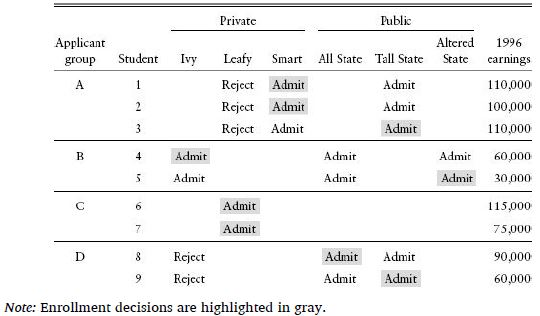
\includegraphics[width=6cm,height=6.5cm,keepaspectratio]{Regression 1} 

\column{.45\textwidth}
\begin{itemize}
	\item Applications, admissions, and matriculation decisions for nine students
	\item E.g.: Group B: Admitted to same schools: Number 4 enrolled at Ivy, while number 5 chose Altered State.
	\item Earnings differential: $30,000 (60 - 30 = 30)$. 
	\item This gap suggests a substantial private school advantage.
\end{itemize}

\end{columns}
\end{frame}

%------------------------------------------------
\begin{frame}
\frametitle{All things equal?}
\begin{itemize}
	\item The Fact, that they were admitted at every school, and just chose different school suggests that they must be pretty similar in their abilities and potential and every earnings gap must be contributed to their school choice.
	\item Using only relevant groups A and B: construct a weighted average: $(\frac{3}{5}\times-5000)+(\frac{2}{5}\times30000)=9000$
	\item By emphasizing larger groups, this weighting scheme uses the data more efficiently and generates a statistically more precise summary of the private-public earnings differential.
	\item Important: apples-to-apples and oranges-to-oranges nature of the underlying matched comparisons: 
		\begin{itemize}
			\item[\rightarrow] Apples in group A are compared to other group A apples, while oranges in group B are compared only with oranges.
		\end{itemize}
\end{itemize}
\end{frame}
%------------------------------------------------
\section{Regression} 
\begin{frame}
\frametitle{The Regression Framework}
\begin{itemize}
	\item regression estimates are weighted averages of multiple matched comparisons
	\item key ingredients in the regression recipe are:
		\begin{itemize}
			\item [\bullet] the dependent variable, in this case, student i’s earnings later in life, also called the outcome variable (denoted by $Y_i$)
			\item [\bullet] the treatment variable, in this case, a dummy variable that indicates students who attended a private college or university (denoted by $P_i$)
			\item [\bullet] a set of control variables, in this case, variables that identify sets of schools to which students applied and were admitted.
		\end{itemize}
	\item Dummies classify data into simple yes-or-no categories
\end{itemize}
	
\end{frame}
%------------------------------------------------
\begin{frame}
\frametitle{The Regression Framework}

\begin{itemize}
	\item The regression model in this context is an equation linking the treatment variable to the dependent variable while holding control variables fixed by including them in the model.
	\item With only one control variable, Ai (if youre group A or not), the regression of interest can be written as: 
	$$Y_i=\alpha+\beta P_i + \gamma A_i + \epsilon_i$$
	\item The regression parameters—called regression coefficients—are:
		\begin{itemize}
			\item[\bullet] the intercept, α (“alpha”);
			\item[\bullet] the causal effect of treatment, β (“beta”);
			\item[\bullet] and the effect of being a group A student, γ (“gamma”)
		\end{itemize}
\end{itemize}

\end{frame}
%------------------------------------------------
\begin{frame}
\frametitle{The Regression Framework}
\begin{itemize}
	\item And there is the residual, $\epsilon_i$ (also called an error term). 
	\item Residuals are defined as the difference between the observed Yi and the fitted values generated by the specific regression model we have in mind. 
	\item These fitted values are written as: 
			$$\hat{Y_i}=\alpha+\beta P_i + \gamma A_i$$
	\item Residuals are given by: 
			$$\epsilon_i=Y_i-\hat{Y_i}=Y_i-(\alpha+\beta P_i + \gamma A_i)

\end{itemize}

\end{frame}
%---------------------------------------------------
\begin{frame}
\frametitle{Explaining the residual}
\begin{columns}
\column{.5\textwidth}
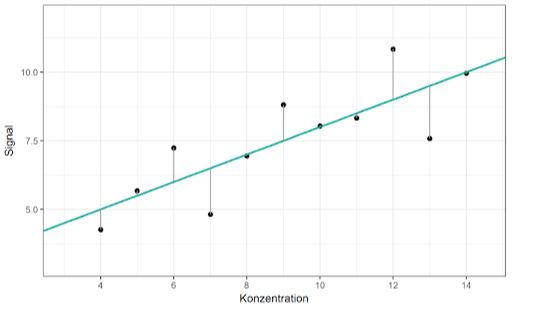
\includegraphics[width=6cm,height=6.5cm,keepaspectratio]{Example Res} 

\column{.45\textwidth}
\begin{itemize}
	\item Difference between the observed value of the dependent variable (Y) and the predicted value $(\hat{Y})$ is the residual
	\item The data points usually don’t fall exactly on this regression equation line; they are scattered around. 	
	\item A residual is the vertical distance between a data point and the regression line.
\end{itemize}
\end{columns}
\end{frame}
%------------------------------------------------

\begin{frame}
\frametitle{Error Term or Residual?}
\begin{itemize}
	\item We must make one important distinction very clear.
	\item The error term (causal language) and the residual (statistical language) are closely related, but not the same.
	\item An error term is the difference between the observed value and the true value, which is unobserved.
	\item So an Error term is a theoretical concept that can never be observed, it is all that explains $Y_i$ and is not included in our regression.
	\item Important: Nothing in our error term can correlate with the treatment, otherwise our causal effect $\beta$ would be confounded by something in the error term.
	\item A residual is the difference between the observed value and the predicted value by our model.
	\item	So the residual is a real world value that is calculated for each time a regression is done.
	
\end{itemize}

\end{frame}

%------------------------------------------------
\begin{frame}
\frametitle{The Regression Framework}
\begin{itemize}
	\item Regression analysis assigns values to model parameters $(\alpha,~ \beta ~and~ \gamma)$ so as to make $\hat{Y_i}$ as close as possible to $Y_i$.
	\item This is accomplished by choosing values that minimize the sum of squared residuals, leading to ordinary least squares (OLS) for the resulting estimates.
	\item This linear regression works under the foundation that that our world can be explained by linear relationships
	\item Important: A regression itself can just tell us something about the statistical correlation, the research design is crucial for our causality.
	\item Regression estimates (and the associated standard errors used to quantify their sampling variance) are readily constructed using computers and econometric software.
	\end{itemize}
\end{frame}

%------------------------------------------------
\begin{frame}
\frametitle{Public-Private Face-Off}

\begin{itemize}
	\item Back to our example of public and private schools: 14,000 former students in the C&B Dataset  made comparable by using the matching matrix
	\item	Because were interested in comparing returns from public and private schools: leaves 5,583 matched students for analysis. These matched students fall into 151 similar selectivity groups containing both public and private students.
	\item New Regression Model:
	$$ln Y_i=\alpha + \beta P_i +\sum^{150}_{j=1}\gamma_i GROUP_{ji} + \delta_1SAT_i +\delta_2 ln PI_i + \epsilon_i$$
\end{itemize}

\end{frame}

%------------------------------------------------
\begin{frame}
\frametitle{Public-Private Face-Off}
\begin{itemize}
	\item Two Changes:
		\begin{itemize}
			\item[\bullet] log of earnings on the left-hand side $\rightarrow$ logged dependent variable allows regression estimates to be interpreted as a percent change.
			\item[\bullet] includes many control variables
		\end{itemize}
	\item The parameter $\beta$ in this model is still the treatment effect of interest, an estimate of the causal effect of attendance at a private school.
	\item $Y_j$, for j = 1 to 150, are the coefficients on 150 selectivity-group dummies, denoted $GROUP{ji}$.
	\item 150 because we need one group as a reference group.
	\item Addition of two further control variables: individual SAT scores ($SAT_i$) and the log of parental income ($PI_i$),
\end{itemize}

\end{frame}

%------------------------------------------------
\begin{frame}
\frametitle{Regressions Run}
\begin{itemize}
	\item We start with regression estimates of the private school earnings advantage from models with no controls.
	\item The coefficient from a regression of log earnings (in 1995) on a dummy for private school attendance, with no other regressors gives the raw difference in log earnings between those who attended a private school and everyone else
	\item Private school students are estimated to have earnings about 14\% higher than the earnings of other students.
	\item Standard errors quantify the statistical precision of the regression estimates reported here. 
\end{itemize}

\end{frame}
%------------------------------------------------
\begin{frame}
\frametitle{Private school effects}
\begin{columns}
\column{.5\textwidth}
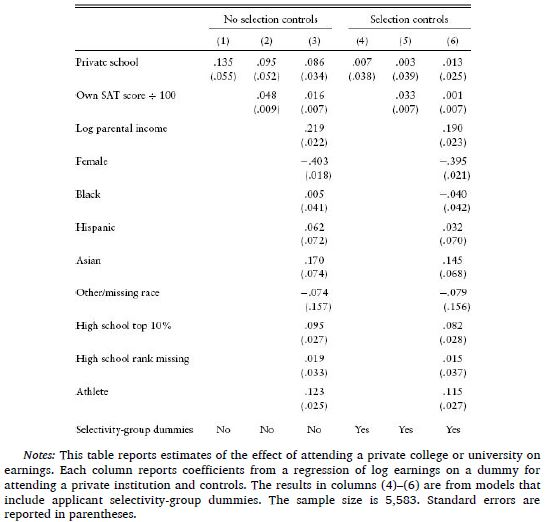
\includegraphics[width=7cm,height=6.5cm,keepaspectratio]{Table 2.2} 

\column{.45\textwidth}
\begin{itemize}
	\item Standard error in column (1) is .055. The Estimate .135 is more than twice the size of the standard error $\rightarrow$ unlikely a chance finding. 
	\item The private school coefficient is statistically significant.
	\item Interesting descriptive fact, but, due to selection bias.
\end{itemize}

\end{columns}
\end{frame}
%------------------------------------------------
\begin{frame}
\frametitle{Private school effects}
\begin{itemize}
	\item Column (2) of Table 2.2: Every 100 points of SAT achievement are associated with a 5 perc. point earnings gain.
	\item Controlling for other factors: brings the private school premium down a little further, to a still substantial and statistically significant .086, reported in column (3) of the table.
	\item Column (4) reports estimates from a model with no controls, but the dummy for each matched college selectivity group in the sample.
	\item The Premium then falls to almost 0, columns (5) and (6) show that the premium moves little when controls for ability and family background are added to the model.
	\item Private university attendance seems unrelated to future earnings once we control for selection bias.
\end{itemize}
\end{frame}

%------------------------------------------------

\begin{frame}
\frametitle{Another Approach}
\begin{columns}
\column{.5\textwidth}
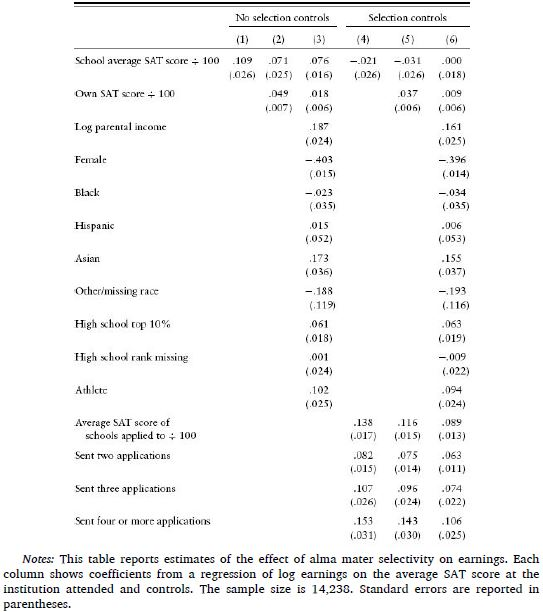
\includegraphics[width=8cm,height=6.5cm,keepaspectratio]{Table 2.4} 

\column{.45\textwidth}
\begin{itemize}
	\item Perhaps our focus on public-private comparisons misses the point. 
	\item Students may benefit from attending schools like Ivy, Leafy, or Smart because their classmates are so much better. 
	\item The synergy generated by a strong peer group may be the feature that justifies the private school price tag.
\end{itemize}

\end{columns}
\end{frame}
%------------------------------------------------
\begin{frame}
\frametitle{Another Approach}
\begin{itemize}
	\item (3) of Table 2.4 show that students who attended more selective schools do markedly better in the labor market, with an estimated college selectivity effect on the order of 8\% higher earnings for every 100 points of average selectivity increase. 
		\begin{itemize}
			\item[\rightarrow] 8\% more earnings per 100 average SAT Score Points
		\end{itemize}
	\item Selection bias due to the greater ambition and ability of those who attend selective schools.
	\item Show average college selectivity to be essentially unrelated to earnings
\end{itemize}

\end{frame}

%------------------------------------------------

\begin{frame}
\frametitle{Ceteris Paribus}
\newline 
\begin{itemize}
	\item Regression is a way to make other things equal, but equality is generated only for variables included as controls on the right-hand side of the model.
	\item Failure to include enough controls or the right controls still leaves us with selection bias.
	\item The regression version of the selection bias generated by inadequate controls is called omitted variables bias (OVB).
\end{itemize}

\end{frame}

%---------------------------------------------------

\begin{frame}
\frametitle{Ceteris Paribus}
\begin{itemize}
	\item Illustration for OVB: Back to the Example of Group A and B:
	\item The “long regression” here includes the dummy variable, Ai, which indicates those in group A. 
	\item We write the regression model that includes $A_i$ as: 
	
	$$Y_i=\alpha^l + \beta^l P_i +\gamma A_i + \epsilon_i^l$$
	
	\item Does the inclusion of $A_i$ matter for estimates of the private school effect in the regression above?
	\item Suppose we make do with a short regression with no controls. This can be written as: 
	$$Y_i=\alpha^s + \beta^s P_i + \epsilon_i^s$$
\end{itemize}

\end{frame}

%---------------------------------------------------
\begin{frame}
\frametitle{Ceteris Paribus}
\begin{itemize}
	\item The Difference between $\beta^s$ and $\beta^l$ is the OVB due to omission of $A_i$ in the short regression. 
	\item Here, OVB amounts to \$10,000, a figure worth worrying about.
	\item Why such a big effect: In part from the fact that the mostly private students in group A have higher earnings anyway, regardless of where they enrolled. 
	\item Inclusion of the group A dummy in the long regression controls for this difference.
\end{itemize}
\end{frame}

%---------------------------------------------------

\begin{frame}
\frametitle{The OVB Formula}
\begin{itemize}
	\item Connection between short and long regression coefficients has two components:
		\begin{itemize}
			\item The relationship between the omitted variable ($A_i$) and the treatment variable ($P_i$); regression of the omitted variable $A_i$ on the private school dummy. 
			$$A_i=\pi_0 + \pi_1 P_i + u_i$$
			
			\item The relationship between the omitted variable ($A_i$) and the outcome variable ($Y_i$). This is given by the coefficient on the omitted variable in the long regression, $\gamma$ 
		\end{itemize}
			\item So we can write the following OVB formula:
			\begin{flalign*}
				OVB &=Effect~ of~ P_i~ in ~short ~- ~Effect~ of~ P_i~ in ~long &\\
				& = \beta^s -\beta^l = \pi_1 \times \gamma 
			\end{flalign*}
\end{itemize}

\end{frame}

%---------------------------------------------------

\begin{frame}
\frametitle{OVB}
\begin{itemize}
	\item Back to our example:
	\item $\pi_1$ in our five-student example is therefore $.1667.$
  \item Calculation of the OVB:
\end{itemize} 
\begin{flalign*}
				OVB &=Short~ -~Long &\\
				& = \beta^s -\beta^l \\
				& = 20.000 -10.000 = 10.000
			\end{flalign*}
and/or 
\begin{flalign*}
				OVB &=Regression ~of ~omitted ~on ~included \times Effect~ of ~omitted~ in ~long &\\
				& = \pi_1 \times \gamma = .1667 \times 60.000 = 10.000
			\end{flalign*}
\end{frame}

%---------------------------------------------------

\begin{frame}
\frametitle{OVB}
\begin{itemize}
	\item OVB formula is a mathematical result that explains differences between regression coefficients in any short-versus-long scenario, irrespective of the causal interpretation of the regression parameters.
	\item The OVB formula is a tool that allows us to consider the impact of control for variables we wish we had. 
	\item This in turn helps us assess whether ceteris is indeed paribus.
	\item We can’t use data to check the consequences of omitting variables that we don’t observe, but we can use the OVB formula to make an educated guess for the consequences of their omission.
\end{itemize}


\end{frame}

%Appendix Corinna
%---------------------------------------------------

\section{Appendix}
\begin{frame}
\frametitle{Regression Sensitivity Analisis}
\begin{itemize}
	\item We might have missed some control variables in our analisis to completely eliminate selection bias
	\item therefore we check how robust our treatment effect is
	\item this means that our treatment effect is insensitive to adding or dropping a particular control variable
	\item as we have seen in the columns (4) - (6) the private school coefficients were insensitve to SAT scores and parental income
	\item this can be explained by the OVB Formula
\end{itemize}

\end{frame}
%---------------------------------------------------

\begin{frame}
\frametitle{Regression Sensitivity Analisis}
\begin{itemize}
	\item short model: regression of log wages on $P_i$ with no controls
	\item long model: adds individual SAT scores
	\item OVB &= ~Short - ~Long = .212 - .152 = .06 (from Table 2.3)
	\item OVB &= Regression ~of ~omitted ~on ~included x Effect~ of ~omitted~ in ~long &= 1.165 x .051 = .06 
\end{itemize}
\end{frame}

%---------------------------------------------------
\begin{frame}
\frametitle{Regression Sensitivity Analisis}
\begin{columns}
\column{.5\textwidth}
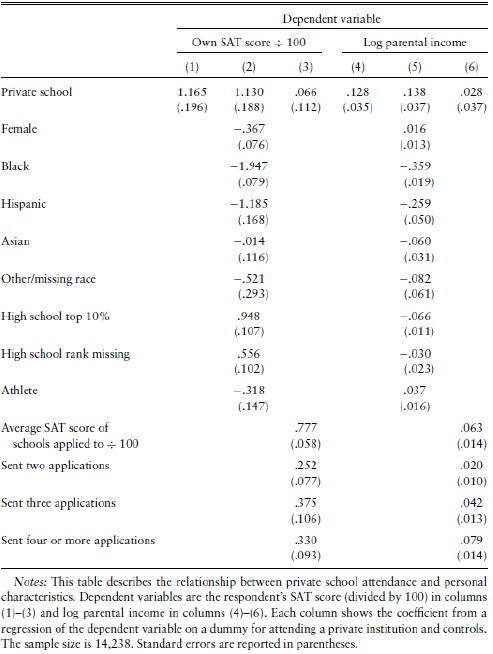
\includegraphics[width=8cm,height=6.5cm,keepaspectratio]{Table 2.5.} 

\column{.45\textwidth}
\begin{itemize}
	\item Relationship between private school attendance and personal characteristics
	\item Regression of omitted on included
	\item Regression of omitted $SAT_i$ on $P_i$
\end{itemize}
\end{columns}
\end{frame}
%---------------------------------------------------


\begin{frame}
\frametitle{Regression Sensitivity Analisis}
\begin{itemize}
	\item short model: regression of log wages on $P_i$ with no controls
	\item long model: adds individual SAT scores
	\item OVB &= ~Short - ~Long = .212 - .152 = .06 (from Table 2.3)
	\item OVB &= Regression ~of ~omitted ~on ~included x Effect~ of ~omitted~ in ~long &= 1.165 x .051 = .06 
	\item when including self-revelation controls, we get
	\item OVB &= ~Short - ~Long = .034 - .031 = .003
	\item OVB &= .066 x .036 = .0024 (instead of .003 due to rounding errors)
	\item students who chose private and public schools aren't very different (at least in SAT scores)
\end{itemize}
\end{frame}

%---------------------------------------------------

\begin{frame}
\frametitle{In a nutshell}
	\begin{itemize}
		\item for causal comparisons we have to compare like with like
		\item good comparisons eliminate systematic differences that are associated with outcomes
		\item the method of matching sorts individuals into groups with the same values of control variables and matched comparisons are averaged
		\item the method of regression is an automated matchmaker
		\item the regression estimate is an average of within-group comparisons
		\item OVB is the difference between short and long regression coefficients
	\end{itemize}

\end{frame}
%---------------------------------------------------

\begin{frame}
\frametitle{Regression and the CEF}
	\begin{itemize}
		\item conditional expectation tell us how the population average of one variable changes as we move the conditioning variable (over the values this variable can assume)
		\item the collection of all such averages is called conditional expectation function (CEF)
		\item the CEF with K conditioning variables is written $$E[Y_i|X_1_i,...,X_K_i]$$
		\item we saw that private school attendance seems to be unrelated to average earnings once certain controls are held fixed
		\item we now suppose that the CEF of log wages is a linear function of these certain conditioning variables, so that:
		\end{itemize}
		$$E[ln Y_i| P_i, GROUP_i, SAT_i, lnPI_i]$$
		$$= \alpha + \beta P_i + \sum{\gamma_j Group_i_i + \delta_1 SAT_i + \delta _ 2 ln PI_i}$$

\end{frame}
%---------------------------------------------------

\begin{frame}
\frametitle{Regression and the CEF}
	\begin{itemize}
		\item when CEF of ln $Y_i$ is a linear funciton of these variables, the regression of ln $Y_i$ recovers this linear funcion
		\item linear models help us to understand regression but regression is even more flexible due to theoretical properties:
		\item If $E[Y_i|X_1_i, ..., X_K_i]= a+\sum_{k=1}^K{{b_kX_k_i}}$ for some constants a and $b1,...,b_K_i$ the regression of $Y_i$ on $X_1_i...., X_K_i$ has intercept a and slope $b1,...,b_k$
		\item if the CEF of $Y_i on X_1_i, ..., X_K_i$ is linear, the regression is it
		\item If $E[Y_i|X_1_i, ..., X_K_i]$ is a nonlinear funcion of the conditioning variables, the rgression of $Y_i$ on $X_1_i, ..., X_K_i$ gives the best linear approximation to this nonlinear CEF
		\item if the CEF is linear, regression finds it and if not, regression finds a good approximation to it
	\end{itemize}
\end{frame}

%--------------------------------------

\begin{frame}
\frametitle{Bivariate Regression and Covariance}
	\begin{itemize}
		\item regression is closely related to the concept variance
		\item the covariance between two variables $X_i$ and $Y_i$ is $$C(X_i,Y_i) = E[(X_i-E[X_i])(Y_i-E[Y_i])]$$
		\item the covariance has three properties:
			\begin{itemize}
				\item covariance of a variable with itself is its variance: $C(X_i,X_i)= \sigma_x^2$
				\item if the expectation of $X_i$ or $Y_i$ is 0, the covariance is the expectation of their product: $C(X_i,Y_i)=E[X_iY_i]$
				\item the covariance between linear functions of $X_i$ and $Y_i$ ($W_i=a+bX_i$ and $Z_i=c+dY_i$) is: $C(W_i,Z_i)=bdC(X_i,Y_i)$
			\end{itemize}
	\end{itemize}

\end{frame}



%---------------------------------------------------

\begin{frame}
\frametitle{Bivariate Regressoin and Covariance}
	\begin{itemize}
		\item a bivariate regression is a regression with one regressor, $X_i$, and an intercept
		\item the bivariate regression slope and intercept are the values of a and b that minimize the residual sum of squares: $$RSS(a,b) = E[Y_i-a-bX_i]^2$$
		\item the solution for the bivariate case is $$b = \beta = \frac{C(Y_i, X_i)}{ V(X_i)}$$ $$a= \alpha = E[Y_i]- \beta E[X_i]$$
		\item when two variables are uncorrelated (covariance of 0), the regression of one on the other generates a slope coefficient of 0!
	\end{itemize}

\end{frame}


%---------------------------------------------------
\begin{frame}
\frametitle{Fits and Residuals}
	\begin{itemize}
		\item regression breaks any dependent variable into two pieces: $Y_i = \^{Y}_i + e_i$
		\item the fitted value $\^{Y}_i$ is the part of $Y_i$ explained by the model and $e_i$ is the residual
		\item regression residuals and regressors are uncorrelated
		\item suppose $\alpha$ and $\beta_1,...,\beta_K$ are the intercept and the slope coefficients of a regression, the fitted values are $$\^{Y}_i = \alpha + \sum_{k=1}^K{{\beta_kX_k_i}}$$ and the regression residuals are \\
		
		$$e_i = Y_i - \^{Y}_i = Y_i - \alpha - \sum_{k=1}^K{{\beta_kX_k_i}}$$
	\end{itemize}

\end{frame}


%---------------------------------------------------
\begin{frame}
\frametitle{Fits and Residuals}
	\begin{itemize}
		\item properties of residuals:
		\item have expectation 0: $E[e_i]=0$
		\item are uncorrelated with all the regressors and with the corresponding fitted values $E[X_k_ie_i]=0$ and $E[\^{Y}_ie_i]=0$
	\end{itemize}

\end{frame}



%---------------------------------------------------
\begin{frame}
\frametitle{Regression for Dummies}
	\begin{itemize}
		\item special case: bivariate regression with a dummy variable
		\item the conditional expectation of $Y_i$ given a dummy $Z_i$ can be $$E[Y_i|Z_i=0]= \alpha $$ and $$E[Y_i|Z_i=1] = \alpha + \beta$$ so that $$\beta = E[Y_i|Z_i=1]-E[Y_i|Z_i=0]$$ 
		\item we can therefore write: $$E[Y_i|Z_i]= E[Y_i|Z_i=0] + (E[Y_i|Z_i=1]-E[Y_i|Z_i=0])Z_i$$
		$$= \alpha + \beta Z_i$$
		\item $E[Y_i|Z_i]$ is a linear function with slope $\beta$ and intercept $\alpha$!
		
	\end{itemize}

\end{frame}


%---------------------------------------------------

\begin{frame}
\frametitle{Regression and OVB}
	\begin{itemize}
		\item A lot of times regressions are multiple and include more control variables
		\item suppose the causal variable is $X_1_i$ and the control variable is $X_2_i$
		\item the coefficient on $X_1_i$ in a regression controlling for $X_2_i$ can be written as:
		$$ \beta_1 = \frac{C(Y_i,\~{X}_1_i)}{V(\~{X}_1_i)}$$ with $\~{X}_1_i$ being the residual from a regression of $X_1_i$ on $X_2_i$ : $$~{X}_1_i= \pi_0 + \pi_1 X_2_i + ~{X}_1_i$$
	\end{itemize}

\end{frame}

%---------------------------------------------------

\begin{frame}
\frametitle{Regression and OVB}
	\begin{itemize}
		\item OVB in multiple regression
		\item call the coefficient on $X_1_i$ in a multivariate regression controlling for $X_2_i$ the long coefficient $\beta^l$: $$Y_i = \alpha^l + \beta ^l X_1_i + \gamma X_2_i + e^l_i$$
		\item call the coefficient in a bivariate regression (without $X_2_i$) $\beta^s$:
		$$Y_i = \alpha^s + \beta ^s X_1_i + e^s_i$$
		\item the OVB would be $\beta^s = \beta^l + \pi_2_1 \gamma$ where $\gamma$ is the coefficient on $X_2_i$ in the long regression and $\pi_2_1$ is the coefficient on $X_1_i$ in a regression of $X_2_i$ on $X_1_i$
		\item short equals long plus the effect of the ommited times the regression of omitted on included!
	
	\end{itemize}

\end{frame}


%---------------------------------------------------
\begin{frame}
\frametitle{Models with Log}
	\begin{itemize}
		\item Let's use a bivariate regression to explain why we use logs instead of just $Y_i$: $$ln Y_i = \alpha + \beta P_i + e_i $$ with $P_i$ being a dummy for private school attendance.
		\item regression in this case fits the CEF perfectly
		\item now we create a ceteris paribus change in $P_i$ for student i: $$ln Y_0_i = \alpha + e_i $$ $$ln Y_1_i = \alpha + \beta + e_i$$
		\item the difference in potential outcomes is therefore $ ln Y_1_i - ln Y_0_i = \beta$
		$$\beta = ln \frac{Y_1_i}{Y_0_i} = ln ( 1+ \frac{Y_1_i - Y_0_i}{Y_0_i} ) $$
		$$= ln ( 1 + \Delta \% Y_p ) \approx \Delta \% Y_p$$
	
	\end{itemize}

\end{frame}

%---------------------------------------------------
\begin{frame}
\frametitle{Models with Log}
	\begin{itemize}
		\item therefore, we can answer the question of why we use logs in regressions as follows:
		\item the regression slope in a model with ln $Y_i$ gives the approximate percentage change in $Y_i$ generated by changing the corresponding regressor
	\end{itemize}

\end{frame}

%---------------------------------------------------

\begin{frame}
\frametitle{Regression Standard Errors and Confidence Intervals}
	\begin{itemize}
		\item the standard error of the slope estimate in a bivariate regression $\hat{\beta}$ is similar to the one we looked at in Chapter 1: $SE(\hat{\beta}) = \frac{\sigma _ e}{\sqrt{n}} x \frac{1}{ \sigma_X}$
		\item $\sigma_e$ is the standard deviation of the regression residuals and $\sigma_X$ is the standard deviation of the regressor
		 \item this formula assumes homoskedasticity meaning that the variance of residuals is unrelated to regressors
	\end{itemize}

\end{frame}

%---------------------------------------------------

\begin{frame}
\frametitle{Regression Standard Errors and Confidence Intervals}
	\begin{itemize}
		\item in case that the homoskedasticity might not be satisfied, meaning we have hetereoskedascity, we need to use robust standard errors:
		$$RSE(\hat{\beta}) = \sqrt{\frac{V(\~X_k_ie_i)}{n(\sigma_{X_k}^2)^2}}$$
	\end{itemize}

\end{frame}


%----------------------------------------------------------------------------------------

\begin{frame}
\Huge{\centerline{Thank you very much for listening}}
\end{frame}

%----------------------------------------------------------------------------------------

\end{document} 